%=========== ΛΥΣΗ - 10ο ΘΕΜΑ Β ===========
\begin{thema}{Β}
Δίνεται η συνάρτηση $f(x) = \dfrac{\ln x + 2}{x}$ με $x > 0$.

\begin{erwthma}
\item Το πεδίο ορισμού της $f$ είναι $D_f = (0, +\infty)$.
Υπολογίζουμε τα όρια στα άκρα του πεδίου ορισμού:
\begin{itemize}
\item $\lim\limits_{x\to0^+} f(x) = \lim\limits_{x\to0^+} \left( (\ln x + 2) \cdot \dfrac{1}{x} \right) = (-\infty) \cdot (+\infty) = -\infty$.
  Επομένως, ο άξονας $y'y$ (ευθεία $x=0$) είναι κατακόρυφη ασύμπτωτη της γραφικής παράστασης $C_f$.
\item $\lim\limits_{x\to+\infty} f(x) = \lim\limits_{x\to+\infty} \dfrac{\ln x + 2}{x} \dlh{\frac{+\infty}{+\infty}} \lim\limits_{x\to+\infty} \dfrac{1}{x} = \lim\limits_{x\to+\infty} \dfrac{1}{x} = 0$.
Επομένως, ο άξονας $x'x$ (ευθεία $y=0$) είναι οριζόντια ασύμπτωτη της $C_f$ στο $+\infty$.
\end{itemize}


\item Η $f(x)$ είναι παραγωγίσιμη στο $(0, +\infty)$ με παράγωγο:
\[ f'(x) = \left( \dfrac{\ln x + 2}{x} \right)' = \dfrac{(\ln x + 2)' x - (\ln x + 2) \cdot (x)'}{x^2} = \dfrac{\dfrac{1}{x}x - (\ln x + 2)}{x^2} = \dfrac{1 - \ln x - 2}{x^2} = \dfrac{-1 - \ln x}{x^2} \]
Για τις ρίζες και το πρόσημο της $f'$:
\begin{itemize}
    \item $f'(x) = 0 \Leftrightarrow \dfrac{-1-\ln x}{x^2} = 0 \Leftrightarrow -1-\ln x = 0 \Leftrightarrow \ln x = -1 \Leftrightarrow x = e^{-1} = \dfrac{1}{e}$
    \item $f'(x) > 0 \Leftrightarrow -1-\ln x > 0 \Leftrightarrow \ln x < -1 \Leftrightarrow x < \dfrac{1}{e}$
    \item $f'(x) < 0 \Leftrightarrow x > \dfrac{1}{e}$
\end{itemize}
Στον παρακάτω πίνακα φαίνεται το πρόσημο της $f'$ και η μονοτονία της $f$:
\begin{center}
\begin{tikzpicture}
\tkzTabInit[color,lgt=2,espcl=1.5,colorC = red7,colorL = red9,colorV = red7]%
{$x$ / .8,$f'(x)$ /0.8,$f(x)$/0.8}%
{$0$,$1/e$,$+\infty$}%
\tkzTabLine{ d, +, z, -, }
\tkzTabVar{ -/,+/,-/ }
\end{tikzpicture}
\end{center}
Άρα η συνάρτηση $f$ είναι γνησίως αύξουσα στο $\left(0, \dfrac{1}{e}\right]$ και γνησίως φθίνουσα στο $\left[\dfrac{1}{e}, +\infty\right)$.
Η συνάρτηση $f$ παρουσιάζει ολικό μέγιστο για $x_0 = \dfrac{1}{e}$, με τιμή:
\[ f(e^{-1}) = \dfrac{\ln(e^{-1}) + 2}{e^{-1}} = \dfrac{-1+2}{e^{-1}} = \dfrac{1}{e^{-1}} = e \]

\item Η $f'(x) = \dfrac{-1-\ln x}{x^2}$ είναι παραγωγίσιμη στο $(0, +\infty)$ με:
\[ f''(x) = \left( \dfrac{-1-\ln x}{x^2} \right)' = \dfrac{(-1-\ln x)' x^2 - (-1-\ln x)(x^2)'}{(x^2)^2} = \dfrac{-\dfrac{1}{x}x^2 - (-1-\ln x)2x}{x^4} \]
\[ = \dfrac{-x + 2x + 2x\ln x}{x^4} = \dfrac{x(1 + 2\ln x)}{x^4} = \dfrac{1 + 2\ln x}{x^3} \]
Για τις ρίζες και το πρόσημο της $f''$:
\begin{itemize}
    \item $f''(x) = 0 \Leftrightarrow 1 + 2\ln x = 0 \Leftrightarrow \ln x = -\dfrac{1}{2} \Leftrightarrow x = e^{-1/2} = \dfrac{1}{\sqrt{e}}$
    \item $f''(x) > 0 \Leftrightarrow 1 + 2\ln x > 0 \Leftrightarrow \ln x > -\dfrac{1}{2} \Leftrightarrow x > \dfrac{1}{\sqrt{e}}$
    \item $f''(x) < 0 \Leftrightarrow 0 < x < \dfrac{1}{\sqrt{e}}$
\end{itemize}
Στον παρακάτω πίνακα φαίνεται το πρόσημο της $f''$ και η κυρτότητα της $f$:
\begin{center}
\begin{tikzpicture}
\tkzTabInit[color,lgt=2,espcl=1.5,colorC = red7,colorL = red9,colorV = red7]%
{$x$ / .8,$f''(x)$ /0.8,$f(x)$/0.8}%
{$0$,$\frac{1}{\sqrt{e}}$,$+\infty$}%
\tkzTabLine{ d, -, z, +, }
\tkzTabLine{ d, \curvearrowright, t, \rotatebox[origin= c]{180}{$\curvearrowleft$}, }
\end{tikzpicture}
\end{center}
Επομένως, η $f$ είναι κοίλη στο $\left(0, \dfrac{1}{\sqrt{e}}\right]$ και κυρτή στο $\left[\dfrac{1}{\sqrt{e}}, +\infty\right)$.
Το σημείο καμπής είναι το $A\left( \dfrac{1}{\sqrt{e}}, f\left(\dfrac{1}{\sqrt{e}}\right) \right)$.
Η τιμή της $f$ στο σημείο αυτό είναι:
\[ f(e^{-1/2}) = \dfrac{\ln(e^{-1/2}) + 2}{e^{-1/2}} = \dfrac{-\dfrac{1}{2} + 2}{e^{-1/2}} = \dfrac{\frac{3}{2}}{\frac{1}{\sqrt{e}}} = \dfrac{3\sqrt{e}}{2} \]
Άρα το σημείο καμπής είναι $A\left( \dfrac{1}{\sqrt{e}}, \dfrac{3\sqrt{e}}{2} \right)$.

\item Για να βρούμε το εμβαδόν του χωρίου από $x=1$ έως $x=e$, πρέπει πρώτα να ελέγξουμε το πρόσημο της $f(x)$ στο διάστημα αυτό.
Για $x \in [1, e]$, είναι $x \ge 1 \Rightarrow \ln x \ge 0 \Rightarrow \ln x + 2 > 0$, οπότε και $\dfrac{\ln x + 2}{x} > 0$. Συνεπώς, $f(x) > 0$.
Άρα το ζητούμενο εμβαδόν είναι:
\[ E = \int_1^e f(x) \d x = \int_1^e \dfrac{\ln x + 2}{x} \d x \]
Θέτουμε $u = \ln x + 2 \Rightarrow \d u = \dfrac{1}{x} \d x$.
\begin{itemize}
\item Για $x = 1 \Rightarrow u = \ln 1 + 2 = 2$
\item Για $x = e \Rightarrow u = \ln e + 2 = 1+2 = 3$
\end{itemize}
Τότε το ολοκλήρωμα γίνεται:
\[ E = \int_2^3 u \d u = \left[ \dfrac{u^2}{2} \right]_2^3 = \dfrac{3^2}{2} - \dfrac{2^2}{2} = \dfrac{9}{2} - \dfrac{4}{2} = \dfrac{5}{2} \]
\end{erwthma}
\end{thema}
%=========== ΤΕΛΟΣ ΛΥΣΗΣ - 10ο ΘΕΜΑ Β ===========
